\section{Alloy}
\subsection{Alloy Model}
In this section will be provided a formal model of the problem achieved using Alloy.
\lstinputlisting[language=alloy]{Alloy/statico.als}
\\

\subsection{World}
\subsubsection{First World}
The 'First World' highlights the role of the students, showcasing their main interactions and relationships within the educational system.
 \begin{figure}[H]
  %\centering
  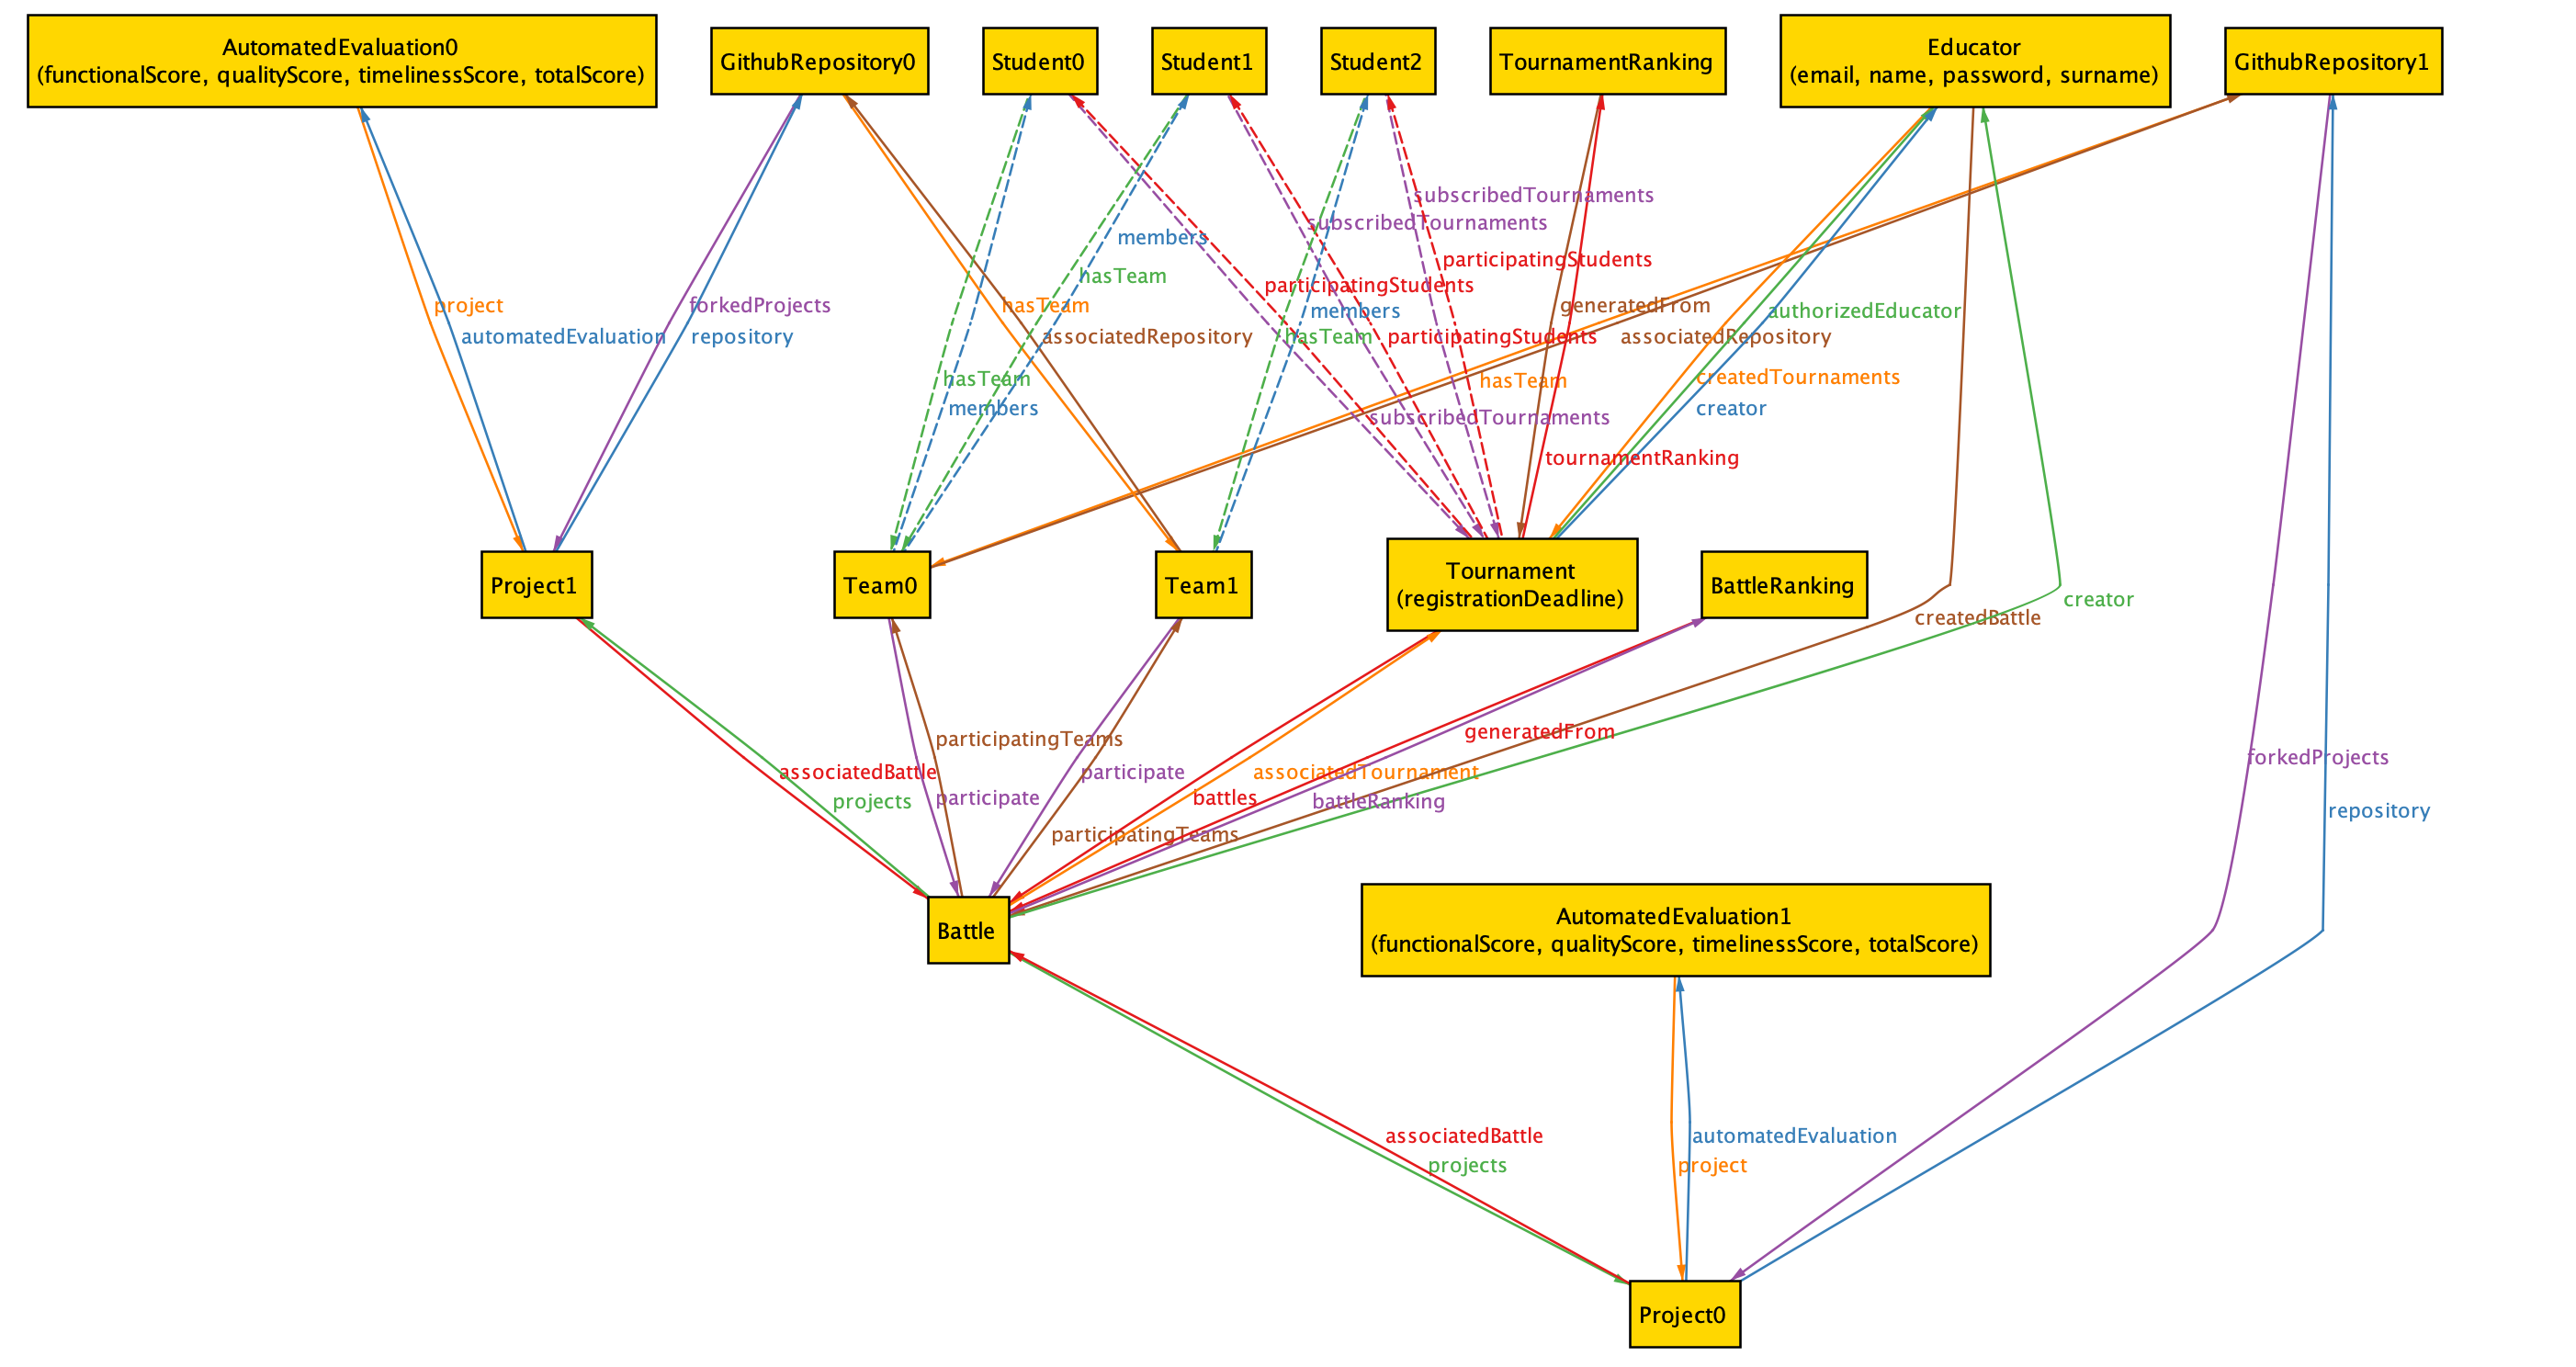
\includegraphics[width=1\linewidth]{Alloy/world1.png} 
  \label{fig:immagine}
\end{figure}

\subsubsection{Second World}
 \begin{figure}[H]
  %\centering
  \includegraphics[width=1\linewidth]{Alloy/world2.png} 
  \label{fig:immagine}
\end{figure}
The 'Second World' emphasizes the role of educators and the methods of evaluation and ranking.

\subsection{Example of dynamic model}
By making the isOpen relationship mutable for the tournament , it is possible to describe the situation in which the tournament is closed by an educator. From that point on, by imposing this fact, it becomes possible to establish that the tournament cannot be reopened. In this Alloy model, we incorporate only the components that differ from the previous model.

\lstinputlisting[language=alloy]{Alloy/loadAlloy.als}